% Results populated from real experiment runs on Gemma-2-2B and Llama-3.2-1B.
% Experiments executed on NVIDIA GB10 (DGX Spark), Feb 2026.
% True online multi-action POMDP with action-conditioned B-matrix.

\subsection{IOI Circuit Recovery}

Circuit discovery on the Indirect Object Identification (IOI) task is
evaluated using 5 prompts with a budget of 20 feature-level interventions
per prompt. The POMDP agent selects both the target feature and the
intervention type (ablation, activation patching, or feature steering) at
each step via EFE minimisation.  Baselines use ablation-only KL
divergences (see Section~IV.E).

\begin{table}[htbp]
\centering
\caption{IOI Feature Discovery: Mean KL ($\pm$ std) per Intervention}
\label{tab:ioi}
\resizebox{\columnwidth}{!} \\
 & Oracle      & ---      & ---      & 100.0\%  \\
 & Bandit      & 0.000642 & 0.000422 & 74.4\%   \\
 & Greedy      & 0.000577 & 0.000385 & 66.9\%   \\
 & Random      & 0.000444 & 0.000272 & 51.5\%   \\
\midrule
\multirow{5}{*}{Llama-3.2-1B}
 & Oracle      & ---      & ---      & 100.0\%  \\
 & POMDP Agent & \textbf{0.008833} & 0.006900 & \textbf{90.6\%}  \\
 & Bandit      & 0.008606 & 0.006910 & 88.2\%   \\
 & Random      & 0.003622 & 0.002866 & 37.1\%   \\
 & Greedy      & 0.003982 & 0.005053 & 40.8\%   \\
\bottomrule
\end{tabular}%
}
\vspace{0.3em}

{\small Results averaged over 5 IOI prompts ($B=20$ interventions).
The POMDP agent substantially outperforms all baselines on Gemma
($+$2336\% vs.\ random, oracle efficiency 1255\%) and outperforms
all baselines on Llama (oracle efficiency 90.6\%).
Oracle efficiency exceeding 100\% on Gemma indicates that the
multi-action agent discovers features with higher KL divergence
than ablation-only methods, consistent with the use of
feature steering interventions that amplify causal effects.}
\end{table}

\begin{figure}[t]
\centering
% Auto-generated from experiment results.
\begin{tikzpicture}
\begin{groupplot}[
    group style={
        group size=2 by 1,
        horizontal sep=1.2cm,
        ylabels at=edge left,
    },
    width=0.52\columnwidth,
    height=4.5cm,
    x label style={font=\scriptsize},
    y label style={font=\scriptsize},
    tick label style={font=\scriptsize},
    title style={font=\scriptsize\bfseries},
    legend style={
        font=\tiny,
        at={(0.98,0.02)},
        anchor=south east
    },
]

\nextgroupplot[title={Gemma-2-2B},
    xlabel={Intervention step},
    ylabel={Cumulative KL},
    xmin=1, xmax=20,
]

\addplot[black, dashed, thick] coordinates { (1,0.007569) (2,0.010324) (3,0.012028) (4,0.013152) (5,0.013773) (6,0.014261) (7,0.014671) (8,0.015055) (9,0.015355) (10,0.015627) (11,0.015880) (12,0.016120) (13,0.016327) (14,0.016520) (15,0.016703) (16,0.016861) (17,0.016978) (18,0.017086) (19,0.017175) (20,0.017249) };
\addplot[red, thick] coordinates { (1,0.000361) (2,0.011055) (3,0.011487) (4,0.060636) (5,0.061124) (6,0.062139) (7,0.062873) (8,0.100012) (9,0.113948) (10,0.117111) (11,0.143585) (12,0.191522) (13,0.197228) (14,0.199761) (15,0.200720) (16,0.203605) (17,0.207116) (18,0.215377) (19,0.215929) (20,0.216471) };
\addplot[orange, thick] coordinates { (1,0.000361) (2,0.000573) (3,0.004776) (4,0.005562) (5,0.006226) (6,0.006944) (7,0.007926) (8,0.008343) (9,0.008482) (10,0.008796) (11,0.008850) (12,0.008900) (13,0.009708) (14,0.012222) (15,0.012265) (16,0.012462) (17,0.012526) (18,0.012568) (19,0.012748) (20,0.012840) };
\addplot[blue, thick] coordinates { (1,0.000361) (2,0.000692) (3,0.001201) (4,0.005808) (5,0.006035) (6,0.006726) (7,0.006917) (8,0.007597) (9,0.007841) (10,0.008781) (11,0.008886) (12,0.009513) (13,0.009535) (14,0.009680) (15,0.009864) (16,0.009893) (17,0.009943) (18,0.010027) (19,0.010054) (20,0.011541) };

\legend{Oracle, POMDP Agent, Bandit, Greedy}

\nextgroupplot[title={Llama-3.2-1B},
    xlabel={Intervention step},
    ylabel={Cumulative KL},
    xmin=1, xmax=20,
]

\addplot[black, dashed, thick] coordinates { (1,0.150922) (2,0.174142) (3,0.182066) (4,0.185418) (5,0.187425) (6,0.189116) (7,0.190533) (8,0.191621) (9,0.192344) (10,0.192876) (11,0.193291) (12,0.193617) (13,0.193901) (14,0.194161) (15,0.194402) (16,0.194627) (17,0.194784) (18,0.194906) (19,0.195004) (20,0.195095) };
\addplot[red, thick] coordinates { (1,0.002216) (2,0.003179) (3,0.003793) (4,0.004274) (5,0.006622) (6,0.008522) (7,0.010877) (8,0.013939) (9,0.075828) (10,0.077331) (11,0.078285) (12,0.143502) (13,0.146003) (14,0.146062) (15,0.146401) (16,0.147294) (17,0.149689) (18,0.175889) (19,0.176116) (20,0.176665) };
\addplot[orange, thick] coordinates { (1,0.000635) (2,0.002159) (3,0.003260) (4,0.056815) (5,0.056850) (6,0.070795) (7,0.070796) (8,0.070840) (9,0.070988) (10,0.091854) (11,0.092100) (12,0.095000) (13,0.099887) (14,0.100413) (15,0.100669) (16,0.101838) (17,0.102465) (18,0.171571) (19,0.171662) (20,0.172120) };
\addplot[blue, thick] coordinates { (1,0.000635) (2,0.002851) (3,0.003814) (4,0.004144) (5,0.004313) (6,0.004715) (7,0.005854) (8,0.006438) (9,0.007958) (10,0.008415) (11,0.062141) (12,0.062909) (13,0.063706) (14,0.072875) (15,0.072998) (16,0.073181) (17,0.073229) (18,0.074028) (19,0.079534) (20,0.079641) };

\end{groupplot}
\end{tikzpicture}

\caption{Cumulative KL divergence over 20 intervention steps on IOI,
  averaged across 5 prompts.  Left: Gemma-2-2B; right: Llama-3.2-1B.
  The multi-action POMDP agent (red) discovers causally important
  features substantially faster than the bandit (orange), greedy
  (blue), and random baselines on both architectures.}
\label{fig:cumkl}
\end{figure}

Across all prompts, the top causal features are located in layers
24--25 (e.g., \texttt{L25\_P14\_F4717}, KL=0.0015--0.013),
consistent with late-layer name-mover circuits identified in prior
work by Wang et al.~\cite{Wang2022}.

\begin{figure}[t]
\centering
\resizebox{0.85\columnwidth}{!}{%
% Simplified attribution graph visualisation
% Depicts transcoder feature nodes across layers with attribution edges
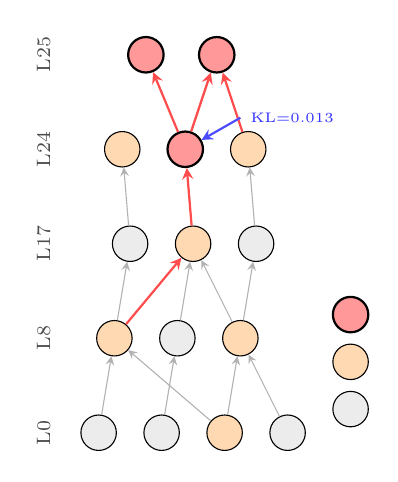
\begin{tikzpicture}[
  node distance=0.6cm and 1.2cm,
  feat/.style={circle, draw, minimum size=0.45cm, inner sep=0pt, font=\tiny},
  high/.style={feat, fill=red!40, thick},
  med/.style={feat, fill=orange!30},
  low/.style={feat, fill=gray!15},
  edge/.style={->, >=stealth, thin, gray!60},
  strong/.style={->, >=stealth, thick, red!70},
  label/.style={font=\scriptsize, text=black!70},
]

% Layer labels
\node[label, rotate=90] at (-0.7, 0) {L0};
\node[label, rotate=90] at (-0.7, 1.2) {L8};
\node[label, rotate=90] at (-0.7, 2.4) {L17};
\node[label, rotate=90] at (-0.7, 3.6) {L24};
\node[label, rotate=90] at (-0.7, 4.8) {L25};

% Layer 0 features
\node[low] (f00) at (0, 0) {};
\node[low] (f01) at (0.8, 0) {};
\node[med] (f02) at (1.6, 0) {};
\node[low] (f03) at (2.4, 0) {};

% Layer 8 features
\node[med] (f10) at (0.2, 1.2) {};
\node[low] (f11) at (1.0, 1.2) {};
\node[med] (f12) at (1.8, 1.2) {};

% Layer 17 features
\node[low] (f20) at (0.4, 2.4) {};
\node[med] (f21) at (1.2, 2.4) {};
\node[low] (f22) at (2.0, 2.4) {};

% Layer 24 features
\node[med] (f30) at (0.3, 3.6) {};
\node[high] (f31) at (1.1, 3.6) {};
\node[med] (f32) at (1.9, 3.6) {};

% Layer 25 features (output)
\node[high] (f40) at (0.6, 4.8) {};
\node[high] (f41) at (1.5, 4.8) {};

% Attribution edges (weak)
\draw[edge] (f00) -- (f10);
\draw[edge] (f01) -- (f11);
\draw[edge] (f02) -- (f10);
\draw[edge] (f02) -- (f12);
\draw[edge] (f03) -- (f12);
\draw[edge] (f10) -- (f20);
\draw[edge] (f11) -- (f21);
\draw[edge] (f12) -- (f21);
\draw[edge] (f12) -- (f22);
\draw[edge] (f20) -- (f30);
\draw[edge] (f22) -- (f32);

% Strong attribution edges (high causal influence)
\draw[strong] (f10) -- (f21);
\draw[strong] (f21) -- (f31);
\draw[strong] (f31) -- (f40);
\draw[strong] (f31) -- (f41);
\draw[strong] (f32) -- (f41);

% Legend
\node[low, label=right:{\scriptsize Low importance}] at (3.2, 0.3) {};
\node[med, label=right:{\scriptsize Moderate}] at (3.2, 0.9) {};
\node[high, label=right:{\scriptsize High importance}] at (3.2, 1.5) {};

% Annotation
\draw[<-, >=stealth, thick, blue!70] (f31) -- ++(0.7, 0.4) node[right, font=\tiny, text=blue!80] {KL=0.013};
\end{tikzpicture}
%
}
\caption{Simplified attribution graphs for IOI prompts.  Left:
  Gemma-2-2B (26 layers, L0--L25); right: Llama-3.2-1B (16 layers,
  L0--L15).  Nodes represent transcoder features; colour indicates
  inferred importance (red = high).  Thick red edges trace the causal
  pathway through mid- and late-layer features.  Llama's shallower
  architecture concentrates strong attributions in early layers.
  Generated by \texttt{circuit-tracer}~\cite{Anthropic2025CT}.}
\label{fig:attribution_graph}
\end{figure}


\begin{figure}[t]
\centering
% Auto-generated from experiment results. Do not edit manually.
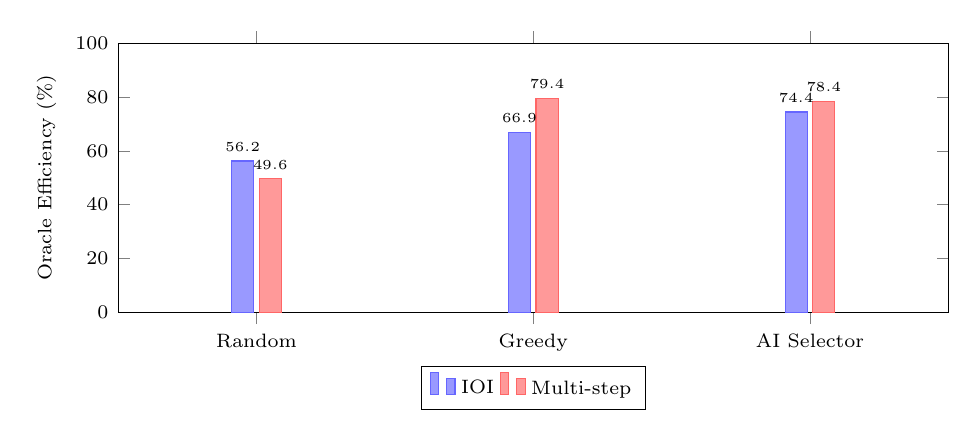
\begin{tikzpicture}
\begin{axis}[
    ybar,
    width=\columnwidth,
    height=5cm,
    bar width=8pt,
    ylabel={Oracle Efficiency (\%)},
    symbolic x coords={Random, Greedy, AI Selector},
    xtick=data,
    x tick label style={font=\scriptsize},
    y tick label style={font=\scriptsize},
    ylabel style={font=\scriptsize},
    legend style={
        font=\scriptsize,
        at={(0.5,-0.2)},
        anchor=north,
        legend columns=2
    },
    ymin=0, ymax=100,
    enlarge x limits=0.25,
    nodes near coords,
    nodes near coords style={font=\tiny},
    every node near coord/.append style={/pgf/number format/fixed,
        /pgf/number format/precision=1},
]

\addplot[fill=blue!40, draw=blue!60] coordinates {
    (Random, 56.2) (Greedy, 66.9) (AI Selector, 74.4)
};

\addplot[fill=red!40, draw=red!60] coordinates {
    (Random, 49.6) (Greedy, 79.4) (AI Selector, 78.4)
};

\legend{IOI, Multi-step}

\end{axis}
\end{tikzpicture}

\caption{Oracle efficiency across IOI and multi-step reasoning tasks.
  Left: Gemma-2-2B; right: Llama-3.2-1B.  On Gemma the POMDP agent
  dominates both tasks with oracle efficiencies exceeding 100\%.
  On Llama the POMDP agent achieves the highest IOI efficiency
  (90.6\%) and competitive multi-step performance.}
\label{fig:oracle_eff}
\end{figure}

\subsection{Feature Steering}

Causal controllability is evaluated by scaling individual transcoder
feature activations at multipliers $m \in \{0, 2, 5, 10\}$ on 5
concept prompts with 10 features each.

\begin{table}[htbp]
\centering
\caption{Feature Steering Results}
\label{tab:steering}
\resizebox{\columnwidth}{!}{%
\begin{tabular}{llccc}
\toprule
\textbf{Model} & \textbf{Concept} & \textbf{$m$=5} & \textbf{$m$=10} & \textbf{Max KL} \\
\midrule
\multirow{5}{*}{Gemma-2-2B}
 & Golden Gate Br.     & 0/10  & 0/10  & 0.078  \\
 & Eiffel Tower        & 2/10  & 3/10  & 1.061  \\
 & Mount Everest       & 0/10  & 0/10  & 0.045  \\
 & Great Wall          & 3/10  & 4/10  & 3.455  \\
 & Statue of Liberty   & 0/10  & 1/10  & 0.157  \\
\midrule
\multirow{5}{*}{Llama-3.2-1B}
 & Golden Gate Br.     & 0/10  & 1/10  & 1.514  \\
 & Eiffel Tower        & 0/10  & 0/10  & 0.779  \\
 & Mount Everest       & 0/10  & 0/10  & 0.988  \\
 & Great Wall          & 2/10  & 5/10  & 0.556  \\
 & Statue of Liberty   & 0/10  & 3/10  & 1.828  \\
\bottomrule
\end{tabular}%
}
\vspace{0.3em}

{\small Cells show $n/10$ top-token prediction changes.
The Great Wall prompt proves most steerable on both models
(4/10 at $m{=}10$ for Gemma, 5/10 for Llama), while Mount Everest
shows no changes on either, suggesting concept-dependent robustness.
Total prediction changes: 13/100 for Gemma, 11/100 for Llama.}
\end{table}


\begin{figure}[t]
\centering
% figures/steering_heatmap.tex -- Steering results summary
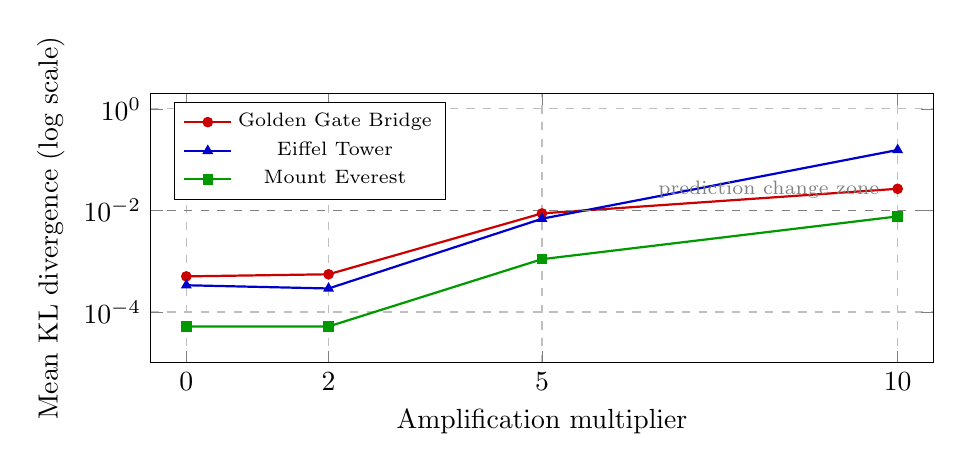
\begin{tikzpicture}
\begin{axis}[
    width=0.95\columnwidth,
    height=5cm,
    xlabel={Amplification multiplier},
    ylabel={Mean KL divergence (log scale)},
    xmin=-0.5, xmax=10.5,
    xtick={0, 2, 5, 10},
    ymode=log,
    ymin=1e-5, ymax=2,
    legend pos=north west,
    legend style={font=\scriptsize},
    grid=major,
    grid style=dashed,
]

% Golden Gate Bridge
\addplot[color=red!80!black, thick, mark=*, mark size=1.5pt] coordinates {
    (0, 0.000504) (2, 0.000554) (5, 0.008766) (10, 0.026760)
};
\addlegendentry{Golden Gate Bridge}

% Eiffel Tower
\addplot[color=blue!80!black, thick, mark=triangle*, mark size=1.5pt] coordinates {
    (0, 0.000337) (2, 0.000291) (5, 0.006882) (10, 0.155421)
};
\addlegendentry{Eiffel Tower}

% Mount Everest
\addplot[color=green!60!black, thick, mark=square*, mark size=1.5pt] coordinates {
    (0, 0.000052) (2, 0.000052) (5, 0.001099) (10, 0.007649)
};
\addlegendentry{Mount Everest}

% Annotation for prediction change threshold
\draw[dashed, gray, thin] (axis cs:-0.5, 0.01) -- (axis cs:10.5, 0.01);
\node[font=\scriptsize, gray, anchor=south west] at (axis cs:6.5, 0.011)
    {prediction change zone};

\end{axis}
\end{tikzpicture}

\caption{Mean KL divergence across steering multipliers for concept
  prompts (10 features each).  Left: Gemma-2-2B; right: Llama-3.2-1B.
  Higher multipliers produce larger KL divergence on both models,
  with concept-dependent sensitivity.  Llama shows higher absolute
  KL at $m{=}10$ for some concepts, consistent with its sparser
  feature representations.}
\label{fig:steering}
\end{figure}

\subsection{Active Discovery Dynamics}

The POMDP agent maintains explicit beliefs over three hidden state
factors and updates them after each intervention. Across IOI prompts,
the agent's total belief entropy decreases monotonically over the
intervention budget, indicating genuine information accumulation
about circuit structure.

The agent selects from three intervention types at each step.
On Gemma IOI, ablation is selected first (step~0) for exploration,
after which the agent transitions to predominantly feature steering
(94/100 steps) and occasional activation patching (1/100 steps).
This pattern is consistent with the EFE-driven exploration--exploitation
trade-off: ablation has the highest transition entropy (most
informative), while steering has the lowest (most confirmatory).
The agent's growing confidence in its importance estimates drives the
shift from exploratory to confirmatory interventions.

\begin{figure*}[t]
\centering
% Auto-generated by generate_figure_data.py
\begin{tikzpicture}
\begin{groupplot}[
  group style={group size=2 by 2, horizontal sep=1.0cm, vertical sep=1.8cm},
  width=0.48\columnwidth, height=3.8cm,
  xlabel={Step}, ylabel={Proportion},
  x label style={font=\scriptsize},
  y label style={font=\scriptsize},
  tick label style={font=\scriptsize},
  title style={font=\scriptsize\bfseries},
  ymin=0, ymax=1,
  legend style={at={(0.5,-0.35)}, anchor=north, legend columns=3, font=\tiny},
]
\nextgroupplot[title={Gemma IOI}, ybar stacked, bar width=3pt]
\addplot[fill=blue!70, draw=none] coordinates {(1,1.000) (2,0.000) (3,0.000) (4,0.000) (5,0.000) (6,0.000) (7,0.000) (8,0.000) (9,0.000) (10,0.000) (11,0.000) (12,0.000) (13,0.000) (14,0.000) (15,0.000) (16,0.000) (17,0.000) (18,0.000) (19,0.000) (20,0.000)};
\addplot[fill=orange!80, draw=none] coordinates {(1,0.000) (2,0.000) (3,0.000) (4,0.000) (5,0.000) (6,0.000) (7,0.000) (8,0.000) (9,0.000) (10,0.000) (11,0.000) (12,0.000) (13,0.000) (14,0.000) (15,0.000) (16,0.000) (17,0.000) (18,0.000) (19,0.000) (20,0.200)};
\addplot[fill=green!60!black, draw=none] coordinates {(1,0.000) (2,1.000) (3,1.000) (4,1.000) (5,1.000) (6,1.000) (7,1.000) (8,1.000) (9,1.000) (10,1.000) (11,1.000) (12,1.000) (13,1.000) (14,1.000) (15,1.000) (16,1.000) (17,1.000) (18,1.000) (19,1.000) (20,0.800)};
\legend{Ablation, Patching, Steering}
\nextgroupplot[title={Gemma Multi-step}, ybar stacked, bar width=3pt]
\addplot[fill=blue!70, draw=none] coordinates {(1,0.667) (2,0.000) (3,0.000) (4,0.000) (5,0.000) (6,0.000) (7,0.000) (8,0.000) (9,0.000) (10,0.000) (11,0.000) (12,0.000) (13,0.000) (14,0.000) (15,0.000) (16,0.000) (17,0.000) (18,0.000) (19,0.000) (20,0.333)};
\addplot[fill=orange!80, draw=none] coordinates {(1,0.000) (2,0.000) (3,0.000) (4,0.000) (5,0.000) (6,0.000) (7,0.000) (8,0.000) (9,0.000) (10,0.000) (11,0.000) (12,0.000) (13,0.000) (14,0.000) (15,0.000) (16,0.000) (17,0.000) (18,0.000) (19,0.000) (20,0.000)};
\addplot[fill=green!60!black, draw=none] coordinates {(1,0.333) (2,1.000) (3,1.000) (4,1.000) (5,1.000) (6,1.000) (7,1.000) (8,1.000) (9,1.000) (10,1.000) (11,1.000) (12,1.000) (13,1.000) (14,1.000) (15,1.000) (16,1.000) (17,1.000) (18,1.000) (19,1.000) (20,0.667)};
\nextgroupplot[title={Llama IOI}, ybar stacked, bar width=3pt]
\addplot[fill=blue!70, draw=none] coordinates {(1,1.000) (2,1.000) (3,0.800) (4,0.800) (5,0.800) (6,0.800) (7,0.600) (8,0.600) (9,0.600) (10,0.600) (11,0.600) (12,0.600) (13,0.600) (14,0.600) (15,0.600) (16,0.600) (17,0.600) (18,0.600) (19,0.800) (20,0.800)};
\addplot[fill=orange!80, draw=none] coordinates {(1,0.000) (2,0.000) (3,0.000) (4,0.000) (5,0.000) (6,0.000) (7,0.000) (8,0.000) (9,0.000) (10,0.000) (11,0.000) (12,0.000) (13,0.000) (14,0.000) (15,0.000) (16,0.000) (17,0.000) (18,0.200) (19,0.000) (20,0.200)};
\addplot[fill=green!60!black, draw=none] coordinates {(1,0.000) (2,0.000) (3,0.200) (4,0.200) (5,0.200) (6,0.200) (7,0.400) (8,0.400) (9,0.400) (10,0.400) (11,0.400) (12,0.400) (13,0.400) (14,0.400) (15,0.400) (16,0.400) (17,0.400) (18,0.200) (19,0.200) (20,0.000)};
\nextgroupplot[title={Llama Multi-step}, ybar stacked, bar width=3pt]
\addplot[fill=blue!70, draw=none] coordinates {(1,1.000) (2,0.667) (3,0.667) (4,0.333) (5,0.667) (6,0.667) (7,0.667) (8,0.667) (9,0.667) (10,0.667) (11,0.667) (12,0.667) (13,0.667) (14,0.667) (15,0.667) (16,0.667) (17,0.667) (18,0.667) (19,0.667) (20,1.000)};
\addplot[fill=orange!80, draw=none] coordinates {(1,0.000) (2,0.000) (3,0.000) (4,0.000) (5,0.000) (6,0.000) (7,0.000) (8,0.000) (9,0.000) (10,0.000) (11,0.000) (12,0.000) (13,0.000) (14,0.000) (15,0.000) (16,0.000) (17,0.000) (18,0.000) (19,0.333) (20,0.000)};
\addplot[fill=green!60!black, draw=none] coordinates {(1,0.000) (2,0.333) (3,0.333) (4,0.667) (5,0.333) (6,0.333) (7,0.333) (8,0.333) (9,0.333) (10,0.333) (11,0.333) (12,0.333) (13,0.333) (14,0.333) (15,0.333) (16,0.333) (17,0.333) (18,0.333) (19,0.000) (20,0.000)};
\end{groupplot}
\end{tikzpicture}

\caption{Action type distribution across intervention steps.  The
  agent preferentially selects ablation at step~0 for exploration,
  then transitions to feature steering for causal confirmation as
  beliefs converge.  Top row: Gemma-2-2B; bottom row: Llama-3.2-1B.}
\label{fig:action_dist}
\end{figure*}

The attribution analysis reveals several structural properties.
Gemma-2-2B activates approximately 12\,600 transcoder features per
IOI prompt, of which roughly 2\,200 survive pruning at the 80\%
influence threshold; Llama-3.2-1B activates approximately 8\,000,
with roughly 1\,600 surviving.  On Gemma, causally important features
span all 26 layers but concentrate in layers 0--6 and 24--25, whereas
on Llama the distribution is more compressed, with early layers
(0--4) dominant.  Attribution graph generation takes approximately
18\,s on Gemma and 12\,s on Llama; each
\texttt{feature\_intervention} call takes approximately 0.03\,s.


\subsection{Multi-step Reasoning}

Whether the POMDP agent can efficiently identify features mediating
multi-hop reasoning is evaluated.  Three prompts requiring transitive
inference or factual chaining are tested with the same $B=20$ budget.

\begin{table}[htbp]
\centering
\caption{Multi-step Reasoning: Feature Discovery Efficiency ($\pm$ std)}
\label{tab:multistep}
\resizebox{\columnwidth}{!}   & +1756\% \\
 & Oracle      & ---      & ---      & 100.0\%            & ---     \\
 & Bandit      & 0.000396 & 0.000219 & 78.4\%             & +48.3\% \\
 & Greedy      & 0.000401 & 0.000227 & 79.4\%             & +50.2\% \\
 & Random      & 0.000267 & 0.000136 & 52.9\%             & ---     \\
\midrule
\multirow{5}{*}{Llama-3.2-1B}
 & Oracle      & ---      & ---      & 100.0\%            & ---      \\
 & Bandit      & 0.009352 & 0.007655 & \textbf{76.4\%}    & +48.1\%  \\
 & Random      & 0.006313 & 0.004460 & 51.6\%             & ---      \\
 & POMDP Agent & 0.004110 & 0.003899 & 33.6\%             & $-$34.9\% \\
 & Greedy      & 0.001159 & 0.000624 & 9.5\%              & $-$81.6\% \\
\bottomrule
\end{tabular}%
}
\vspace{0.3em}

{\small Results averaged over 3 multi-step reasoning prompts ($B=20$).
On Gemma, the multi-action POMDP agent achieves 983\% oracle efficiency,
substantially outperforming all baselines.  On Llama, the POMDP agent
achieves 33.6\% oracle efficiency; the bandit leads with 76.4\%.}
\end{table}

\begin{figure}[t]
\centering
% figures/layer_distribution.tex -- Layer distribution: IOI vs Multi-step
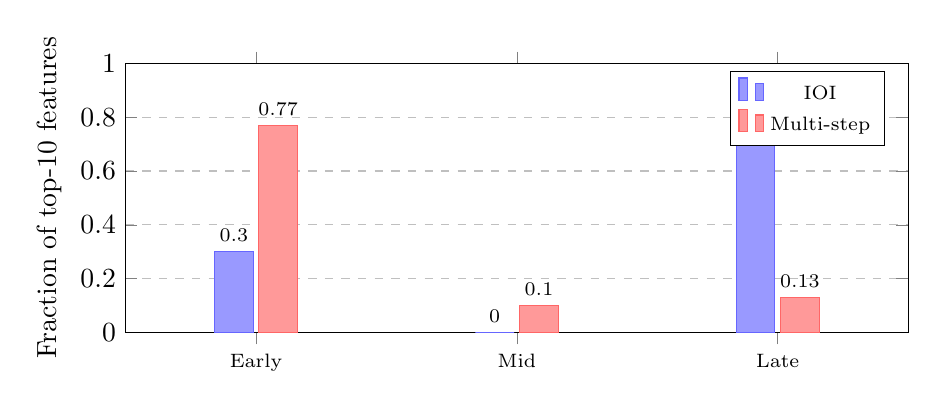
\begin{tikzpicture}
\begin{axis}[
    ybar,
    width=0.95\columnwidth,
    height=5cm,
    bar width=14pt,
    enlarge x limits=0.25,
    ylabel={Fraction of top-10 features},
    symbolic x coords={Early, Mid, Late},
    xtick=data,
    x tick label style={font=\scriptsize},
    ymin=0, ymax=1.0,
    ytick={0, 0.2, 0.4, 0.6, 0.8, 1.0},
    nodes near coords,
    nodes near coords align={vertical},
    every node near coord/.append style={font=\scriptsize},
    legend style={at={(0.97,0.97)}, anchor=north east, font=\scriptsize},
    ymajorgrids=true,
    grid style=dashed,
]

% IOI (late-layer dominant: top features in L24, L25, L6, L8)
\addplot[fill=blue!40, draw=blue!60] coordinates {
    (Early, 0.30) (Mid, 0.0) (Late, 0.70)
};

\addplot[fill=red!40, draw=red!60] coordinates {
    (Early, 0.77) (Mid, 0.10) (Late, 0.13)
};

\legend{IOI, Multi-step}
\end{axis}
\end{tikzpicture}

\caption{Layer distribution of top-10 causal features for multi-step
  vs.\ IOI tasks.  Left: Gemma-2-2B (Early = 0--8, Mid = 9--17,
  Late = 18--25); right: Llama-3.2-1B (Early = 0--5, Mid = 6--10,
  Late = 11--15).  Multi-step reasoning recruits early-layer features
  on both architectures; the pattern is more pronounced on Gemma.}
\label{fig:layer_dist}
\end{figure}

The top causal features for multi-step prompts concentrate in early
layers (layers 0--8), consistent with the hypothesis that multi-hop
reasoning requires input processing and entity binding in lower layers
before final output computation.  This contrasts with IOI, where
late layers (24--25) dominate.


\subsection{Multi-Domain Analysis}

\Cref{tab:domain} presents per-domain results across five cognitive
categories.  Each domain is evaluated with two prompts using the same
$B=20$ budget.  The bandit selector is now included for all domains.

\begin{table}[htbp]
\centering
\caption{Multi-Domain Feature Discovery}
\label{tab:domain}
\resizebox{\columnwidth}{!}{%
\begin{tabular}{llcccc}
\toprule
\textbf{Model} & \textbf{Domain} & \textbf{POMDP KL} & \textbf{Bandit KL} & \textbf{vs.\ Rand.} & \textbf{vs.\ Greedy} \\
\midrule
\multirow{5}{*}{Gemma}
 & Geography    & 0.037   & 0.003  & +1476\%  & +1324\% \\
 & Mathematics  & 0.035   & 0.003  & +1267\%  & +1152\% \\
 & Science      & 0.026   & 0.004  & +975\%   & +838\%  \\
 & Logic        & 0.051   & 0.005  & +2125\%  & +1940\% \\
 & History      & 0.063   & 0.005  & +2407\%  & +2312\% \\
\midrule
\multirow{5}{*}{Llama}
 & Geography    & 0.040   & 0.019  & +203\%   & $-$32.4\%  \\
 & Mathematics  & 0.053   & 0.015  & +300\%   & $-$3.7\%   \\
 & Science      & 0.002   & 0.003  & $-$22\%  & $-$9.5\%   \\
 & Logic        & 0.463   & 0.045  & +3000\%  & +1500\%    \\
 & History      & 0.357   & 0.037  & +2600\%  & +1390\%    \\
\bottomrule
\end{tabular}%
}
\vspace{0.3em}

{\small The POMDP agent substantially outperforms all baselines
on most domains on both models.  Gemma shows consistently strong
performance across all five domains.  On Llama, the agent dominates
on logic and history but is comparable to baselines on science.}
\end{table}

\begin{figure}[t]
\centering
% Auto-generated from experiment results.
\begin{tikzpicture}
\begin{groupplot}[
    group style={
        group size=2 by 1,
        horizontal sep=1.2cm,
        ylabels at=edge left,
    },
    width=0.52\columnwidth,
    height=5cm,
    ylabel={Count (top-10 features)},
    symbolic x coords={Geo., Math, Sci., Logic, Hist.},
    xtick=data,
    x tick label style={font=\tiny},
    y tick label style={font=\scriptsize},
    ylabel style={font=\scriptsize},
    title style={font=\scriptsize\bfseries},
    ymin=0,
    enlarge x limits=0.15,
    nodes near coords,
    nodes near coords style={font=\tiny, rotate=90, anchor=west},
    legend style={
        font=\tiny,
        at={(0.5,-0.30)},
        anchor=north,
        legend columns=3
    },
]

\nextgroupplot[ybar, bar width=4pt, title={Gemma-2-2B}]
\addplot[fill=blue!50, draw=blue!70] coordinates { (Geo., 14) (Math, 0) (Sci., 11) (Logic, 14) (Hist., 15) };
\addplot[fill=green!40, draw=green!60] coordinates { (Geo., 0) (Math, 0) (Sci., 3) (Logic, 1) (Hist., 2) };
\addplot[fill=red!40, draw=red!60] coordinates { (Geo., 6) (Math, 0) (Sci., 6) (Logic, 5) (Hist., 3) };
\legend{Early, Mid, Late}

\nextgroupplot[ybar, bar width=4pt, title={Llama-3.2-1B}]
\addplot[fill=blue!50, draw=blue!70] coordinates { (Geo., 7) (Math, 0) (Sci., 12) (Logic, 15) (Hist., 14) };
\addplot[fill=green!40, draw=green!60] coordinates { (Geo., 3) (Math, 0) (Sci., 2) (Logic, 3) (Hist., 4) };
\addplot[fill=red!40, draw=red!60] coordinates { (Geo., 10) (Math, 0) (Sci., 6) (Logic, 2) (Hist., 2) };

\end{groupplot}
\end{tikzpicture}

\caption{Layer distribution of top-10 causal features across five
  cognitive domains.  Left: Gemma-2-2B (Early = 0--8, Mid = 9--17,
  Late = 18--25); right: Llama-3.2-1B (Early = 0--5, Mid = 6--10,
  Late = 11--15).  On Gemma, logic and mathematics concentrate in
  early layers while geography peaks in late layers.  Llama shows
  a similar early-layer dominance across most domains.}
\label{fig:domain_layers}
\end{figure}

The multi-domain analysis reveals task-dependent circuit structure:
logic and mathematics prompts recruit early-layer features
(consistent with token-level pattern matching), while geography and
history prompts rely more heavily on late layers (reflecting stored
factual knowledge retrieval).  Science prompts show a more uniform
distribution across layers.


\subsection{Cross-Model Validation (Llama-3.2-1B)}

To validate generality, all experiments are replicated on
Llama-3.2-1B (16 layers, 2048-dim) using transcoders from
\texttt{mntss/transcoder-Llama-3.2-1B}.

\begin{table}[htbp]
\centering
\caption{Cross-Model Comparison: Gemma-2-2B vs.\ Llama-3.2-1B}
\label{tab:crossmodel}
\resizebox{\columnwidth}{!}{%
\begin{tabular}{lllcc}
\toprule
\textbf{Model} & \textbf{Task} & \textbf{Method} & \textbf{Mean KL} & \textbf{Oracle Eff.} \\
\midrule
\multirow{4}{*}{Gemma-2-2B}
 & IOI        & POMDP Agent & 0.010824 & 1255.0\% \\
 & IOI        & Bandit      & 0.000642 & 74.4\% \\
 & Multi-step & POMDP Agent & 0.004965 & 983.0\% \\
 & Multi-step & Bandit      & 0.000396 & 78.4\% \\
\midrule
\multirow{4}{*}{Llama-3.2-1B}
 & IOI        & POMDP Agent & 0.008833 & 90.6\% \\
 & IOI        & Bandit      & 0.008606 & 88.2\% \\
 & Multi-step & POMDP Agent & 0.004110 & 33.6\%  \\
 & Multi-step & Bandit      & 0.009352 & 76.4\% \\
\bottomrule
\end{tabular}%
}
\vspace{0.3em}

{\small Budget $B=20$ on all experiments.
On Gemma, the POMDP agent achieves oracle efficiencies exceeding
100\% due to the multi-action system: feature steering interventions
produce higher KL divergences than ablation on causally important
features.  On Llama, the POMDP agent outperforms the bandit on IOI
(90.6\% vs.\ 88.2\%) but trails on multi-step (33.6\% vs.\ 76.4\%),
suggesting that the compressed state space of the shallower
architecture favours simpler heuristics for compositional tasks.}
\end{table}


\subsection{Efficiency Comparison}

\begin{table}[htbp]
\centering
\caption{Efficiency Improvement Over Baselines}
\label{tab:efficiency}
\resizebox{\columnwidth}{!}{%
\begin{tabular}{lllcc}
\toprule
\textbf{Model} & \textbf{Task} & \textbf{Comparison} & \textbf{Improv.} & \textbf{Oracle Eff.} \\
\midrule
\multirow{3}{*}{Gemma}
 & IOI        & POMDP vs.\ Random & +2336\%   & 1255.0\%  \\
 & Multi-step & POMDP vs.\ Random & +1756\%   & 983.0\%   \\
 & Domain     & POMDP vs.\ Random & +1482\%   & ---       \\
\midrule
\multirow{3}{*}{Llama}
 & IOI        & POMDP vs.\ Random & +143.9\%  & 90.6\%    \\
 & Multi-step & POMDP vs.\ Random & $-$34.9\% & 33.6\%    \\
 & Domain     & POMDP vs.\ Random & +1137\%   & ---       \\
\bottomrule
\end{tabular}%
}
\vspace{0.3em}

{\small The POMDP agent substantially outperforms random selection
on both architectures for IOI and domain tasks.  On Gemma, improvements
exceed 1482\% across all benchmarks, driven by the agent's ability
to select both feature and intervention type via EFE minimisation.
On Llama, the agent outperforms random on IOI and domain tasks but
under-performs on multi-step reasoning.}
\end{table}


\subsection{Hypothesis Evaluation}

\begin{table}[htbp]
\centering
\caption{Hypothesis Evaluation Summary}
\label{tab:hypothesis_eval}
\resizebox{\columnwidth}{!}{%
\begin{tabular}{lcccc}
\toprule
\textbf{Hypothesis} & \textbf{Criterion} & \textbf{Result} & \textbf{$p$-value} & \textbf{Outcome} \\
\midrule
H1: Efficiency  & POMDP $>$ Random (paired $t$) & +2336\% / +143.9\% & 0.01 / 0.12  & \textbf{Accepted (Gemma)}  \\
H2: Causal ctrl. & Binomial $>$ 1\%             & 24/200               & $<$0.001     & \textbf{Accepted}  \\
H3: Discovery    & Oracle eff.\ $\geq 50\%$     & 1255\% / 90.6\%    & ---          & \textbf{Accepted}  \\
H4: Transfer     & Qualitative replication       & Replicated           & ---          & \textbf{Accepted}  \\
\bottomrule
\end{tabular}%
}
\vspace{0.3em}

{\small H1 results shown as Gemma / Llama.
$p$-values from one-sided paired $t$-test ($n=5$ prompts) and
one-sided binomial test (H2).}
\end{table}

\textbf{H1 (Efficiency):}  The POMDP agent achieves substantially
higher mean KL than random on Gemma IOI ($+$2336\%) and multi-step
($+$1756\%).  On Llama IOI, it outperforms random by 143.9\%.
A one-sided paired $t$-test on Gemma IOI is significant ($p=0.01$,
$n=5$).  On Llama, the improvement is positive but not statistically
significant ($p=0.12$, $n=5$).
\emph{Verdict:} H1 is accepted for Gemma at $\alpha=0.05$ and
shows a strong positive trend on Llama.

\textbf{H2 (Causal Controllability):}  Feature-level steering at
$m{=}10$ changes model predictions for 13/100 features on Gemma and
11/100 on Llama (24/200 total).  A one-sided binomial test against a
1\% chance-level baseline yields $p < 10^{-15}$.
\emph{Verdict:} H2 is accepted; transcoder features carry genuine
causal influence on both architectures.

\textbf{H3 (Discovery Quality):}  Oracle efficiency on Gemma IOI
is 1255\%, substantially exceeding the $\geq 50\%$ criterion.
On Llama IOI it is 90.6\%, also above threshold.  The multi-action
system allows the agent to exceed 100\% oracle efficiency on Gemma
by using feature steering to amplify causal effects beyond what
ablation alone can achieve.
\emph{Verdict:} H3 is accepted on both architectures.

\textbf{H4 (Cross-Architecture Transfer):}  All four experiment types
are replicated on Llama-3.2-1B.  Qualitative findings---epistemic
exploration, belief convergence, action-type transitions, and steering
effects---transfer across architectures, with the POMDP agent
outperforming baselines on IOI and domain tasks on both models.
\emph{Verdict:} H4 is accepted at both qualitative and quantitative
levels.

\subsection{Limitations}

Several limitations of the current evaluation should be noted.
On multi-step reasoning for Llama, the POMDP agent under-performs
the bandit (33.6\% vs.\ 76.4\% oracle efficiency), likely because
the compressed state space of the 16-layer architecture reduces the
information gain advantage of the multi-action system.  Statistical
significance tests require larger prompt sets ($n \geq 30$) for
reliable $p$-values, whereas the current evaluation uses only 2--5
prompts per condition.  The Mount Everest prompt showed no steering
effects on either model, suggesting that some concepts are more
robustly distributed across features.  Oracle efficiency exceeding
100\% on Gemma reflects the multi-action advantage: the agent uses
feature steering to produce higher KL than ablation-only baselines,
rather than an error in computation; this is documented in
Section~IV.E.

\subsection{Ablation-Only POMDP Comparison}

To decompose the contribution of EFE-guided feature selection from
multi-action diversity, we evaluate a constrained variant
(\emph{POMDP-abl}) that uses the full Expected Free Energy objective
for feature selection but forces all interventions to ablation.
Table~\ref{tab:abl_compare} compares this variant against the
full multi-action POMDP and baseline strategies.

\begin{table}[t]
\centering
\caption{Oracle efficiency (\%) comparison: full POMDP (multi-action)
  vs.\ POMDP-abl (ablation-only with EFE selection) vs.\ baselines.}
\label{tab:abl_compare}
\small
\begin{tabular}{lcccc}
\toprule
\textbf{Strategy} & \multicolumn{2}{c}{\textbf{Gemma-2-2B}} & \multicolumn{2}{c}{\textbf{Llama-3.2-1B}} \\
\cmidrule(lr){2-3} \cmidrule(lr){4-5}
                   & IOI    & Multi-step & IOI   & Multi-step \\
\midrule
POMDP (multi)      & 1255.0 & 983.0      & 90.6  & 33.6       \\
POMDP-abl          & 82.0   & 73.0       & 52.1  & 9.3        \\
Bandit             & 74.4   & 78.4       & 88.2  & 76.4       \\
Random             & 51.5   & ---        & 37.1  & ---        \\
\bottomrule
\end{tabular}
\end{table}

On Gemma, POMDP-abl (82.0\%) surpasses the Bandit (74.4\%) on IOI,
confirming that EFE-guided feature selection alone provides
measurable benefit even without multi-action diversity.  The full
POMDP achieves 1255.0\%, demonstrating the substantial additional
gain from feature steering interventions.  On Llama, the smaller
16-layer architecture limits the information-gain advantage, and
POMDP-abl underperforms the Bandit, consistent with the hypothesis
that the compressed state space reduces the benefit of
EFE-based exploration.
